\section{Methods}

\subsection{Overall framework}

    To implement the permanent set model (chapter 4) for numerical simulations, we will utilize the effective constitutive model approach (chapter 5). This implementation has 4 main components (Fig. \ref{c6:fig:pssimoverview}): 1) initial state model, 2) quasistatic simulation, 3) updates to the material properties in response to permanent set and 4) updates to the finite element model geometry in response to permanent set. 
    
    
%%%%%%%%%%%%%%%%%%%%%%%%%%%%%%%%%%%%%%%%%%%%%%%%%%%%%%%%%%%%
%-------------------	begin FIGURE 	-------------------%
\begin{figure}
\centering
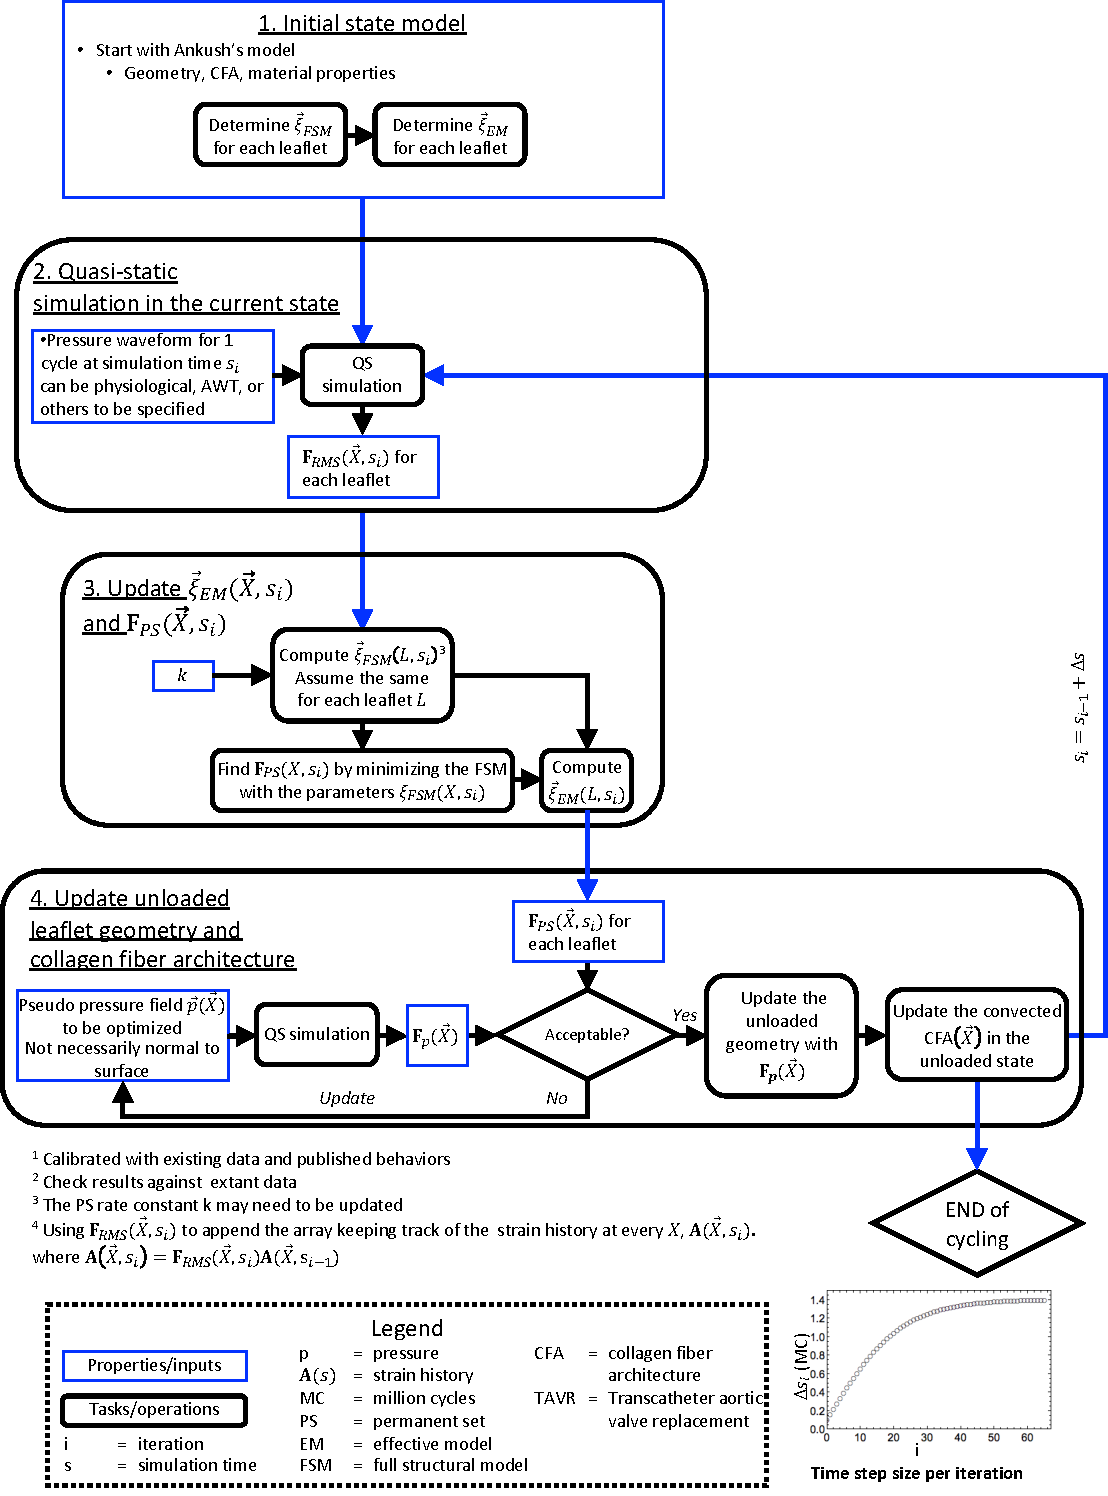
\includegraphics[width=5.5in]{Images/chapter6/pssimoverview.pdf}
\caption{Proposed frame work for simulation the evolving properties of BHVs in response to permanent set.}
\label{c6:fig:pssimoverview}
\end{figure}
%-------------------	 end FIGURE 	-------------------%
%%%%%%%%%%%%%%%%%%%%%%%%%%%%%%%%%%%%%%%%%%%%%%%%%%%%%%%%%%%%

\subsection{Initial state model}

    In this part the initial parameters of the simulation is established. The 3 main components are: 1) finite element mesh for BHV geometry, 2) leaflet material properties, and 3) mapped collagen fiber architecture. For the BHV geometry, our group developed a pipline using micro-CT to measure the 3-dimensional geometry of the BHV and fitting the atrial surface points to a NURBS mesh using the grash hopper plugin in Rhino (Copyright Robert McNeel \& Associates) (Fig. \ref{c6:fig:fegeometry}). We also previously developed an approach for mapping the collagen fiber architecture to the finite element mesh \cite{aggarwal_patient_2013,aggarwal_inverse_2015}. However, due to the lack of available experimental data, we used the Edwards valve geometry from \cite{aggarwal_inverse_2015}, bovine pericardium material properties from \cite{sacks_novel_2016}, and circumferential aligned collagen fiber orientation distributions.
    
%%%%%%%%%%%%%%%%%%%%%%%%%%%%%%%%%%%%%%%%%%%%%%%%%%%%%%%%%%%%
%-------------------	begin FIGURE 	-------------------%
\begin{figure}
\centering
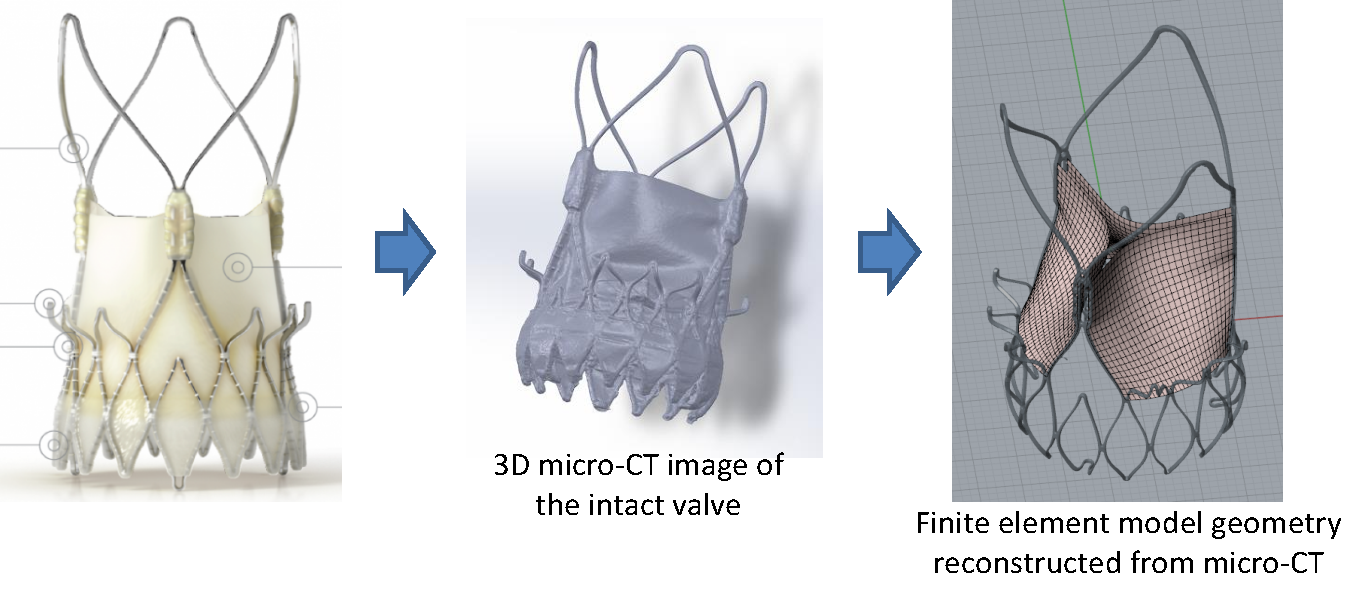
\includegraphics[width=5.5in]{Images/chapter6/fegeometry.pdf}
\caption{Pipeline for converting micro-CT data for each reference and loading states to finite element meshs and geometry.}
\label{c6:fig:fegeometry}
\end{figure}
%-------------------	 end FIGURE 	-------------------%
%%%%%%%%%%%%%%%%%%%%%%%%%%%%%%%%%%%%%%%%%%%%%%%%%%%%%%%%%%%%

\subsection{Quasistatic simulation of bioprosthetic heart valves}

	For the quasistatic simulation, which is necessary to determine the current loaded state, we will utilized the effective model approach (Fig. \ref{c6:fig:simulationframework}) established in chapter 5. For finite element model, we utilized the custom finite element simulation software developed by Hsu \textit{et al.} \cite{hsu_dynamic_2015, kamensky_immersogeometric_2015, kiendl_isogeometric_2015, wu_anisotropic_2018}. Briefly, the finite element code was developed for isogeometric fluid solid dynamics simulation of heart valves, focusing mostly on the tri-leaflet atrioventricular valves. The tri-leaflet geometry is based on the commonly used Edwards Pericardial Heart Valve with Kirchhoff-Love shells for the leaflets \cite{kiendl_isogeometric_2015} and finite element solver developed in by Kamensky \textit{et al.} \cite {kamensky_immersogeometric_2015}. We utilized this code to simulate leaflet deformation under physiological quasi--static transvalvular pressure. 
    A total was 484 B\'ezier elements was used for each leaflets, with a leaflet density of 1.0 g/cm$^3$ and a uniform leaflet thickness of 0.386mm thick \cite{hsu_dynamic_2015}. Contact between leaflets is handled by a penalty-based approach and imposed at quadrature points of the shell structure, and clamped boundary condition is applied to the leaflet attachment edge. 
    For simplicity and consistency, the collagen fiber direction was assume to be aligned to the circumferential direction of each leaflet. No root, atrial chamber or the surrounding artery was used. The bioprothetic heart valve stent was made rigid and undeformable, serving a stationary reference for the leaflets. A similar validation process to the one presented by Wu \textit{et al.} \cite{wu_anisotropic_2018} to verify the implementation.
	
	
	For the constitutive model for the leaflet material, we used the effective material model (chapter 5)
	%==========================================================%
%-------------------	begin EQUATION 	-------------------%
\begin{equation} \label{c6:eqn:finalexponentialmodelformscaled}
\begin{aligned}
\Psi_{eff} 	=& c_0 \left(e^{Q} - 1\right) = c_0^\prime e^{-Q_{max}}\left(e^{Q} - 1\right)    \\
Q		=& b_1 E_m^2 + b_2 E_n^2 + b_3 E_\phi^2 + b_4 E_m E_n + b_5 E_m^4 + b_6 E_n^4 + b_7 E_m^3 E_n + b_8 E_m^2 E_n^2 \\ 
&+ b_9 E_m E_n^3 + b_{10} E_\phi^4 + b_{11} E_m^2E_\phi^2 + b_{12} E_n^2 E_\phi^2 + b_{13} E_m E_n E_\phi^2 \\
Q		=& b_1 (E_m^{max})^2 + b_2 (E_n^{max})^2 + b_3 (E_\phi^{max})^2 + b_4 (E_m^{max}) (E_n^{max}) + b_5 (E_m^{max})^4   \\
    &+ b_6 (E_n^{max})^4 + b_7 (E_m^{max})^3 (E_n^{max}) + b_8 (E_m^{max})^2 (E_n^{max})^2 + b_9 (E_m^{max}) (E_n^{max})^3	\\
	&+ b_{10} (E_\phi^{max})^4 + b_{11} (E_m^{max})^2(E_\phi^{max})^2 + b_{12} (E_n^{max})^2 (E_\phi^{max})^2    \\ 
	&+ b_{13} (E_m^{max}) (E_n^{max}) (E_\phi^{max})^2,
\end{aligned}
\end{equation}
%-------------------	 end EQUATION 	-------------------%
%==========================================================%
	to homogenize the mechanical response of the permanent set model. The resulting elasticity tensor for can be found in Appendix \ref{sec:elasticitytensor}, Eqn. \ref{eqn:greenelasticityform}). To test the finite element implementation, and the effective constitutive model approaches, we performed several quasi-static simulations of BHVs with different leaflet materials properties. The main properties considered are bovine pericardium (most commonly used for bioprothetic heart valve leaflets), porcine aortic valve (highly anisotropy response), and bovine pericardium with an uniform fiber ODF (isotropic). We replicated the response of these tissues using the static part of the permanent set constitutive model for collagenous soft tissues (Eqn. \ref{c6:structuralmodelcomponents}) based on their microstructure. We then fit $\Psi_{eff}$ (Eqn. \ref{c6:eqn:finalexponentialmodelformscaled}) their response by sampling along optimal loading paths. Next, we evaluated the computational cost and numerical robustness of $\Psi_{eff}$ and its ability to handle a wide range of material properties and the complex \textit{in vivo} deformations in numerical simulations.
    

\subsection{Constitutive model for the evolving material properties under permanent set}

    The detailed theory for the constitutive model for permanent set is presented in chapter 4. Briefly, the constitutive model consists of three parts: collagen, matrix, and interactions,
%==========================================================%
%-------------------	begin EQUATION 	-------------------%
\begin{equation}
\Psi 	= \Psi_\mathrm{col} + \Psi_\mathrm{mat} + \Psi_\mathrm{int} \label{c6:eqn:structuralmodelcomponents}. 
\end{equation}
%-------------------	 end EQUATION 	-------------------%
%==========================================================%
    The time evolving mechanism is based on the work by Rajagopal and Wineman \cite{rajagopal_constitutive_1992}, where we assume that the response of the EXL matrix is a constrained mixture model consisting of the origin fraction being continuously converted to new fractions with a reference state in the current loaded configuration. 
\begin{equation} \label{c6:eq:wineman}
\phi_m \mathbf{S}_m = b(s)\mathbf{\bar{S}}_m^\mathrm{existing} + \int\displaylimits_0^s a(s,\hat{s})\mathbf{\bar{S}}_m^\mathrm{new} \mathrm{d}\hat{s},
\end{equation}

    The final model form as a function of the permanent set rate constant $k $, the permanent set deformation $\mathbf{F}_\mathrm{PS}$, the strain history $\mathbf{A}(s)$, and the material parameters of the constitutive model in the uncycled state. The input of the model is the applied deformation $\mathbf{C}$ referenced to the current unloaded state $\Omega_\mathrm{PS}$, given by the deformation $\mathbf{F}_\mathrm{PS}$ from $\Omega_0$. The full form is
\begin{equation}\label{c6:eq:fullEXLmodel}
\mathbf{S} = \mathbf{S}\left(k , \mathbf{F}_\mathrm{PS}, \mathbf{A}(\hat{s}), \mathbf{C}\right) = \phi_\mathrm{col} \left[ \mathbf{S}_\mathrm{col} + \mathbf{S}_\mathrm{int}\right] + \phi_m \mathbf{S}_\mathrm{m},
\end{equation}
where the collagen contribution is 
\begin{equation} \label{c6:eq:fullcollagen}
\begin{split}
\phi_\mathrm{col}\mathbf{S}_\mathrm{col}&\left(k , \mathbf{F}_\mathrm{PS}, \mathbf{A}(\hat{s}), \mathbf{C}\right) \\
&= \phi_\mathrm{col} \eta_C \int\displaylimits_\theta \Gamma_1(\mathbf{F}_{\mathrm{PS}}, \theta)\left\lbrace 
\int\displaylimits_1^{\lambda_\theta} \frac{D_1\left( \mathbf{F}_{\mathrm{PS}}, x \right)}{x} \left( \frac{1}{x}- \frac{1}{\lambda_\theta}\right) \mathrm{d}x \right\rbrace \mathbf{n}_\theta\otimes\mathbf{n}_\theta \mathrm{d}\theta,
\end{split}
\end{equation}
where $\lambda_\theta = \sqrt{\mathbf{n}_\theta \cdot \mathbf{C}\mathbf{n}_\theta}$ is the stretch of the fiber ensemble oriented along $\theta$, the fiber ensemble interactions is 
\begin{equation} \label{c6:eq:fullinteractions}
\begin{split}
\phi_\mathrm{int}\mathbf{S}_\mathrm{int}&\left(k , \mathbf{F}_\mathrm{PS}, \mathbf{A}(\hat{s}), \mathbf{C}\right) \\
=& \phi_\mathrm{col} \eta_\mathrm{int} \int\displaylimits_\alpha \int\displaylimits_\beta \Gamma_1 \left(\mathbf{F}_\mathrm{PS}, \alpha \right) \Gamma_1 \left(\mathbf{F}_\mathrm{PS},  \beta \right) \\
&\times\left[ \left\lbrace 
\int\displaylimits_1^{\lambda_\alpha} \int\displaylimits_1^{\lambda_\beta} 
\frac{2 \lambda_\beta D_1(\mathbf{F}_\mathrm{PS}, x_\alpha) D_1(\mathbf{F}_\mathrm{PS}, x_\beta)}{x_\alpha x_\beta} 
\left( \frac{\lambda_\alpha}{x_\alpha} \frac{\lambda_\beta}{x_\beta} - 1\right) \mathrm{d}x_\alpha \, \mathrm{d}x_\beta \right.\right. \\
&+ \left. \left. \int\displaylimits_1^{\lambda_\beta} D_1(\mathbf{F}_\mathrm{PS}, x_\beta) \left( \frac{\lambda_\beta}{x_\beta} -1  \right)^2 \mathrm{d}x_\beta \right\rbrace \right.  \frac{\mathbf{n}_\alpha \otimes \mathbf{n}_\alpha}{\lambda_\alpha}  \\
&+ \left. \left\lbrace
\int\displaylimits_1^{\lambda_\alpha} \int\displaylimits_1^{\lambda_\alpha} 
\frac{2 \lambda_\beta D_1(\mathbf{F}_\mathrm{PS}, x_\alpha) D_1(\mathbf{F}_\mathrm{PS}, x_\beta)}{x_\alpha x_\beta} 
\left( \frac{\lambda_\alpha}{x_\alpha} \frac{\lambda_\beta}{x_\beta} - 1\right) \mathrm{d}x_\alpha \, \mathrm{d}x_\beta 
\right. \right. \\
&+\left. \left. \int\displaylimits_1^{\lambda_\alpha} D_1(\mathbf{F}_\mathrm{PS}, x_\alpha) \left( \frac{\lambda_\alpha}{x_\alpha} -1  \right)^2 \mathrm{d}x_\alpha \right\rbrace \frac{\mathbf{n}_\beta \otimes \mathbf{n}_\beta}{\lambda_\beta}  \right] \mathrm{d}\alpha \, \mathrm{d}\beta,
\end{split}
\end{equation}
and the EXL matrix is
\begin{equation} \label{c6:eq:fullmatrix}
\begin{split}
\phi_m \mathbf{S}_\mathrm{m}&\left(k , \mathbf{F}_\mathrm{PS}, \mathbf{A}(\hat{s}), \mathbf{C}\right) \\
&= \phi_m \eta_m \left[ \vphantom{\int\displaylimits_0^s} \mathrm{Exp}\left[-k  \cdot s\right]  \left(\left( \bar{I_1} (\mathbf{F}_\mathrm{PS}, \mathbf{A}(0)) - 3\right)^{\alpha - 1} + r \left( \bar{I_1} (\mathbf{F}_\mathrm{PS}, \mathbf{A}(0)) - 3\right)^{\beta - 1}\right)  \right.\\
&\times \left( \mathbf{\tilde{B}}(\mathbf{F}_\mathrm{PS}, \mathbf{A}(0))^{-1} - \tilde{B}_{33}^{-1}(\mathbf{F}_\mathrm{PS}, \mathbf{A}(0))C_{33}\mathbf{C}^{-1}\right) \\
&+ \int\displaylimits_0^s k \cdot \mathrm{Exp}\left[-k (s - \hat{s})\right] \left(\left( \bar{I_1} (\mathbf{F}_\mathrm{PS}, \mathbf{A}(\hat{s})) - 3\right)^{\alpha - 1} + r \left( \bar{I_1} (\mathbf{F}_\mathrm{PS}, \mathbf{A}(\hat{s})) - 3\right)^{\beta - 1}\right) \\
&\times \left. \vphantom{\int\displaylimits_-^s} \left( \mathbf{\tilde{B}}(\mathbf{F}_\mathrm{PS}, \mathbf{A}(\hat{s}))^{-1} - \tilde{B}_{33}^{-1}(\mathbf{F}_\mathrm{PS}, \mathbf{A}(\hat{s}))C_{33}\mathbf{C}^{-1}\right) \mathrm{d}\hat{s}\right].
\end{split}
\end{equation}

\subsection{Geometry update in response to permanent set}

    Although the permanent set model can find the local change in reference geometry, ($\mathbf{F}_\mathrm{PS}$), can be determined from equation \ref{c6:eq:fullmatrix} using
\begin{equation}\label{c6:eq:optimization}
\begin{gathered}
\mathbf{F}_\mathrm{PS} = \operatorname*{arg\,min}_\mathbf{F} \left\Vert \mathbf{S}\left(k , \mathbf{I}, \mathbf{A}(\hat{s}), \mathbf{C}=\mathbf{F}^\mathsf{T}\mathbf{F}\right) - 0 \right\Vert.
\end{gathered}
\end{equation}
    This is only local and will not be sufficient for generating a compatible mesh. To generate the updated reference configuration, we will do this by simulation. First the local change in geometry is found (Eqn. \ref{c6:eq:optimization}). Next, we will compute an equivalent stress using equation \ref{c6:eq:fullEXLmodel}, by
\begin{equation}\label{c6:eq:psstress}
\begin{gathered}
\mathbf{S}_\mathrm{PS} = \mathbf{S}(\mathbf{F}_\mathrm{PS}).
\end{gathered}
\end{equation}
    This permanent set stress, $\mathbf{S}_\mathrm{PS}$, is equivalent of a growth stress, which is then added to the weak form presented in equation 1 of Wu et al. \cite{wu_anisotropic_2018} as 
\begin{equation}\label{c6:eq:weakform}
\begin{aligned}
\int_{\Gamma_0} \mathbf{w}\cdot\rho h_{th} \left.\dpd[2]{y}{t}\right|_\mathbf{X} \dif\Gamma + 
\int_{\Gamma_0} \int_{-h_{th}/2}^{h_{th}/2}\delta\mathbf{E}:(\mathbf{S} + \mathbf{S}_\mathrm{PS}) \dif \xi^3\dif\Gamma&  \\
- \int_{\gamma_0} \mathbf{w}\cdot\rho h_{th}\mathbf{f}\dif\Gamma -\int_{\Gamma_t} \mathbf{w}\cdot\mathbf{h}\dif\Gamma = 0&
\end{aligned}
\end{equation}   
    The resulting control point displacements are then added to the finite element mesh from the previous time step to generate the new mesh in the new reference configuration. 
    

\subsection{Complete implementations with Python wrapper}

    The complete implementation of the time evolving simulation is done using a Python3 wrapper (Fig. \ref{c6:fig:pythonimplementation}) of the different components: 
    \begin{enumerate}[label=\Alph*]
        \item Quasi-static (QS) simulation code to obtain the NURBS control point displacement data for different loading conditions
        \item A post processor for translate displacement data to strain data at each gauss point
        \item The constitutive model for determine the change in material properties due to permanent set gauss point
        \item Parameter estimation code for determining the effective model parameters at each time step and gauss point
        \item Python code for updating the NURBS finite element mesh after each time step
        \item Python code for updating the collagen fiber orientation after each time step
    \end{enumerate}
    To start, we will use the Edwards valve geometry from \cite{aggarwal_inverse_2015}, bovine pericardium material properties from \cite{sacks_novel_2016}, and circumferential aligned collagen fiber orientation distributions. Next, the following process are iterated:
    \begin{enumerate}
        \item Perform QS simulation using the finite element code to determine the loading state
        \item Using the post processor to convert control point displacement data to local strain data, $\mathbf{A}(\Hat{s})$, at the current time $\Hat{s}$
        \item Append the strain in the loaded configuration, $\mathbf{A}(\Hat{s})$, to the full strain history $\mathbf{A}(s)$
        \item Update the permanent set constitutive model (Eqn. \ref{c6:eq:fullEXLmodel})
        \item Use equation \ref{c6:eq:fullEXLmodel} to compute the local $\mathbf{F}_\mathrm{PS}$, 
        $\mathbf{S}_\mathrm{PS}$, and mechanical data along optimal loading paths (chapter \ref{sec:optimaldesign})
        \item Use the local permanent set deformation to convect the collagen fiber orientation distribution $\Gamma_i$ in the current state to $\Gamma_{i+1}$ in the post permanent set state using 
        %-------------------	begin EQUATION 	-------------------%
        \begin{equation}\label{c6:eqn:45}
        \begin{aligned}
        \Gamma_{i+1}[\mu_\Gamma,\sigma_\Gamma, \theta_{i+1}] = \Gamma_i[\mu_\Gamma, \sigma_\Gamma, \theta_i(\prescript{i+1}{i}{\mathbf{F}},\theta_{1+1})\frac{\prescript{i+1}{i}{\lambda}_{\theta_i}^2}{\prescript{i+1}{i}{J_\mathrm{2D}}}].
        \end{aligned}
        \end{equation}
        %-------------------	 end EQUATION 	-------------------%
        Note that the angle $\theta_1$ of a fibre originally oriented at $\theta_0$ can be determined using
        %-------------------	begin EQUATION 	-------------------%
        \begin{equation}\label{c6:eqn:46}
        \begin{aligned}
        \theta_{i+1}(\prescript{i+1}{0i}{\mathbf{F}},\theta_i) = \tan^{-1}\left(\frac{\prescript{i+1}{i}{F}_{21}\cos{\theta_i} + \prescript{i+1}{i}{F}_{22}\sin{\theta_i}}{\prescript{i+1}{i}{F}_{11}\cos{\theta_i} + \prescript{i+1}{i}{F}_{12}\sin{\theta_i}}\right)
        \end{aligned}
        \end{equation}
        %-------------------	 end EQUATION 	-------------------%
        \item[7a] Perform QS simulation using the finite element code with $\mathbf{S}_\mathrm{PS}$ as the loading condition
        \item[7b] Added the control point displacement data to the current mesh geometry
        \item[8] Determine the new effective constitutive model parameters by performing parameter estimation on the optimal loading path data using equation \ref{c6:eqn:finalexponentialmodelformscaled}
        \item[9] Go to step 1 and rerun the QS simulation using the new mesh geometry, effective constitutive model parameters, and collagen fiber architecture
    \end{enumerate}
    This loop is run for the desired number of cycles. 
%%%%%%%%%%%%%%%%%%%%%%%%%%%%%%%%%%%%%%%%%%%%%%%%%%%%%%%%%%%%
%-------------------	begin FIGURE 	-------------------%
\begin{sidewaysfigure}
\centering
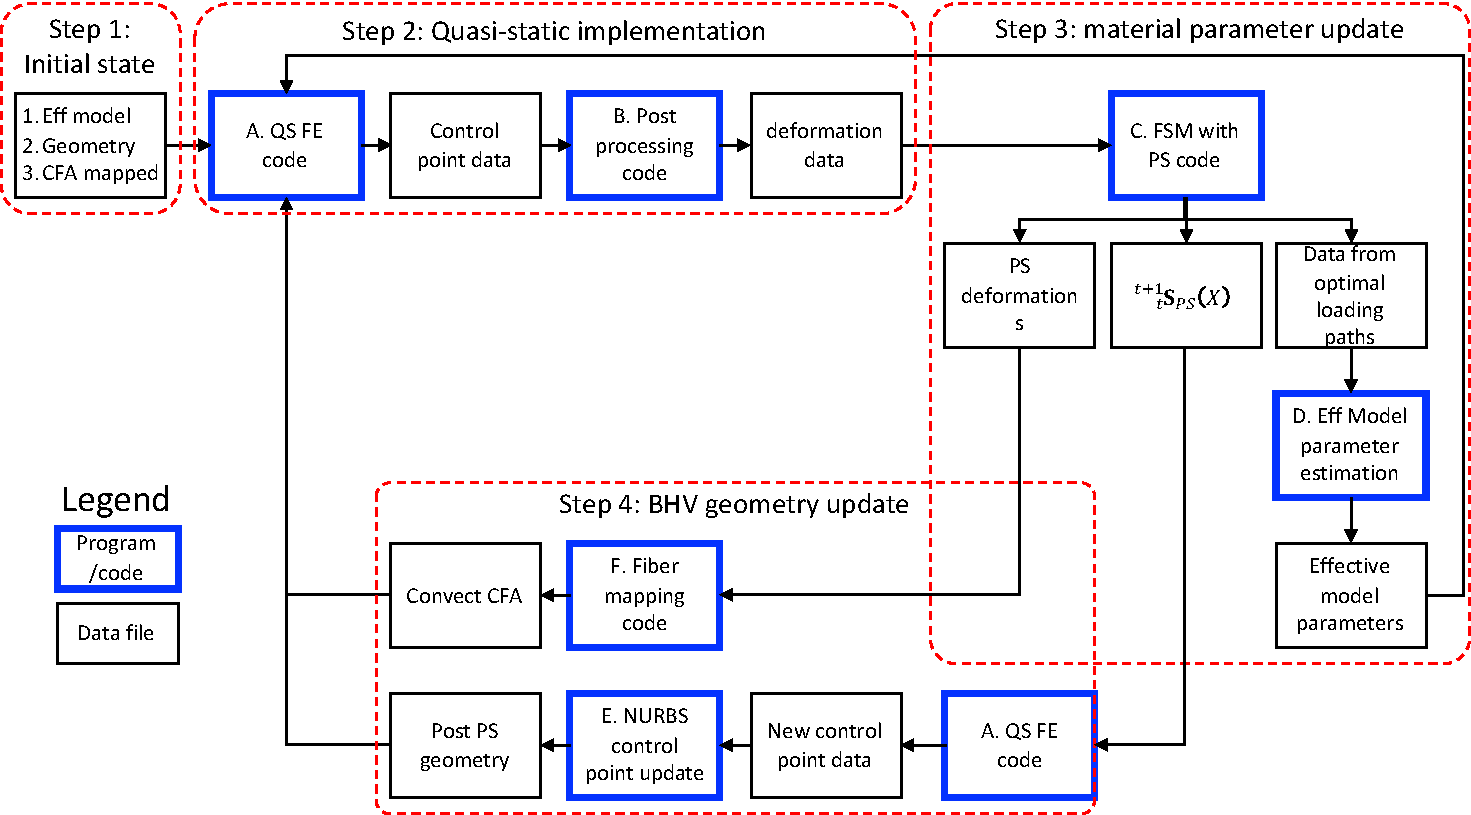
\includegraphics[width=8.2in]{Images/chapter6/pythonimplementation.pdf}
\caption{The python wrapper for communicating and execution of the different component of the time dependent simulation framework.}
\label{c6:fig:pythonimplementation}
\end{sidewaysfigure}
%-------------------	 end FIGURE 	-------------------%
%%%%%%%%%%%%%%%%%%%%%%%%%%%%%%%%%%%%%%%%%%%%%%%%%%%%%%%%%%%%